\chapter{Verification}\label{Verification chapter}
In this chapter we will verify implementations of the algorithm presented in chapter \ref{method_chap} using the discretization detailed in chapter \ref{disc_chap}. All implementations are done in the Python programming language, and the numerics is done using the NumPy\cite{walt2011numpy} library. Plots are created using the matplotlib\cite{Hunter:2007} package, tables are auto generated using Pandas\cite{mckinney2010data} and the parallel parts are implemented using the mpi4py\cite{dalcin2007mpi4py} library. We test our algorithm using the example problem (\ref{exs_J}-\ref{exs_E}), with the following parameters:
\begin{align}
&J(y,v) = \frac{1}{2}\int_0^1v(t)^2dt + \frac{1}{2}(y(1)-11.5)^2 \label{test_J}\\
&\left\{
     \begin{array}{lr}
       	y'(t) = -3.9y(t)+v(t) \ t\in(0,1)\\
       	y(0)=3.2
     \end{array}
   \right. \label{test_E}
\end{align}
Using this problem we will first test the numerical gradients stated in section \ref{num_grad_sec1} and \ref{num_grad_sec2}, and then investigate if the minimizer of the discretized objective function converges to the exact minimizer derived in section \ref{exact_sec}. We also check if the theoretical speedup for objective function and gradient evaluation suggested in \ref{analysis sec} is in line with actual measurements. The last test done is on the consistency of the penalty framework. 
\section{Taylor Test} \label{Taylor_sec}
The Taylor test is a good way to test the correctness of the gradient of a function. The test is as its name implies connected with Taylor expansions of a function, or more precisely the following two observations:
\begin{align*}
|J(v+\epsilon w)-J(v)| &= \mathcal{O}(\epsilon) \\
|J(v+\epsilon w)-J(v)-\epsilon\nabla J(v)\cdot w| &= \mathcal{O}(\epsilon^2)
\end{align*}
Here $w$ is a vector in the same space as $v$, while $\epsilon>0$ is a constant. The test is carried out by evaluating $D=|J(v+\epsilon w)-J(v)-\epsilon\nabla J(v)\cdot w|$ for decreasing $\epsilon$'s, and if $D$ approaches 0 at 2nd order rate, we consider the test as passed.
\subsection{Verifying the Numerical Gradient Using the Taylor Test}
We will now use the Taylor test on the discrete gradient stemming from problem (\ref{test_J}-\ref{test_E}). We discretize this problem using the Crank-Nicolson scheme for the state and adjoint equation, and the trapezoid rule for numerical integration, as suggested in chapter \ref{disc_chap}. We let the time step be $\Delta t=\frac{1}{100}$, and evaluate the objective function and its gradient using the control variable $v=1$. To apply the Taylor test, we need a direction $w\in\mathbb{R}^{101}$, which we set to be a vector with components randomly chosen from numbers between 0 and 100. To make table \ref{Taylor_tab1} more readable we define the following measures:
\begin{align}
D_1(\epsilon) &= |J(v+\epsilon w)-J(v)| \label{D1} \\
D_2(\epsilon) &=|J(v+\epsilon w)-J(v)-\epsilon \nabla J(v)\cdot w|\label{D2}
\end{align} 
We evaluate $D_1(\epsilon)$ and $D_2(\epsilon)$ for decreasing $\epsilon$s, and list the results in table \ref{Taylor_tab1}.
\\
\begin{table}[h]
\caption{Results from Taylor test conducted on non-penalized discrete objective function. $\epsilon$ is the decreasing parameter used in $D_1(\epsilon)$ (\ref{D1}) and $D_2(\epsilon)$ (\ref{D2}). The last two columns of the table show the rate at which $D_1(\epsilon)$ and $D_2(\epsilon)$ approach zero for decreasing $\epsilon$. If $D_2(\epsilon)$ converges to zero at second order rate the test is passed, and this is indeed observed in the results of the table. }
\label{Taylor_tab1}
\centering
\begin{tabular}{lrrrll}
\toprule
{} $\epsilon$&  $D_1$ &  $D_2$ &        $||\epsilon w||_{l_{\infty}}$ &    $ \log(\frac{D_1(\epsilon)}{D_1(10\epsilon)})$ &    $ \log(\frac{D_2(\epsilon)}{D_2(10\epsilon)})$ \\
\midrule
1.0e+00 &  5956.494584 &        5.24e+03 &  99.987417 &       -- &       -- \\
1.0e-01 &   123.645671 &        5.24e+01 &   9.998742 &  -1.7 &  -2 \\
1.0e-02 &     7.644529 &        5.24e-01 &   0.999874 &  -1.2 &  -2 \\
1.0e-03 &     0.717253 &        5.24e-03 &   0.099987 &  -1.0 &  -2 \\
1.0e-04 &     0.071253 &        5.24e-05 &   0.009999 &  -1.0 &  -2 \\
1.0e-05 &     0.007121 &        5.24e-07 &   0.001000 &  -1.0 &  -2 \\
1.0e-06 &     0.000712 &        5.24e-09 &   0.000100 &  -1.0 &  -2 \\
1.0e-07 &     0.000071 &        5.25e-11 &   0.000010 &  -1.0 &  -2 \\
\bottomrule
\end{tabular}
\end{table}
\\
\\
Table \ref{Taylor_tab1} clearly shows that $|J(v+\epsilon w)-J(v)-\epsilon \nabla J(v)\cdot w|$ converges to zero at a second order rate. This means that the numerical gradient of our test problem passes the Taylor test. This again indicates that both the numerical gradient and the implementation of it are correct. We include a plot of the gradient used in the Taylor test together with a finite difference approximation of $\hat J'(v)$ in figure \ref{JGrad1}. We see that the discrete gradient form section \ref{DiscGradSec1} is practically identical to the finite difference approximation. Notice also how the discrete gradient have jumps in its first and last component. These jumps come from the discretization method used on the integral, the state equation and adjoint equation. Next we check whether the gradient of the discrete and penalized objective function passes the Taylor test.
\begin{figure}[h]
\centering
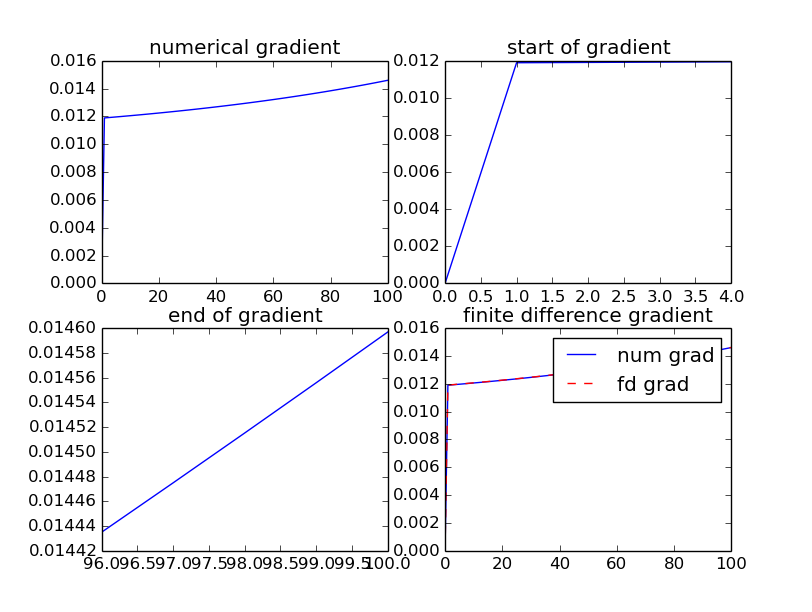
\includegraphics[scale=0.5]{num_grad.png}
\caption{Gradient of non-penalized objective function of problem (\ref{test_J}-\ref{test_E}) calculated using expression from section \ref{num_grad_sec1}, and a finite difference approximation. Notice that these methods produce almost identical results. The jumps at $t=0$ and $t=1$, are numerical artefacts stemming from the Crank-Nicolson and trapezoid rule discretization of the objective function.}
\label{JGrad1}
\end{figure}
\subsection{Verifying the Penalized Numerical Gradient Using the Taylor Test}
We will now use the Taylor test on the penalized numerical gradient (\ref{num_pen_grad_lam}-\ref{num_pen_grad_v}) that we get when decomposing $I=[0,T]$ into $N=10$ subintervals while solving the same problem as in the test for the gradient of the non-penalized objective function (\ref{test_J}-\ref{test_E}). We then discretize in time using $\Delta t=\frac{1}{100}$. The control variable is now a vector $v\in\mathbb{R}^{N+m}$ and we set $v_k=0 \ \forall k=0,...,N+n-1$, while the $w_k$s are chosen randomly from numbers between 0 and 100. The results of applying the Taylor test to this problem are given in table \ref{Taylor_tab2}. Here $D_1$ and $D_2$ are again defined as in (\ref{D1}-\ref{D2}).
\\
\begin{table}[!h]
\centering
\caption{Taylor test for penalized discrete objective function. We are again interested in at what rate $D_1(\epsilon)$ and $D_2(\epsilon)$ converge to zero, when we decrease $\epsilon$. We observe that $D_1(\epsilon)$ approaches zero at a first order rate, while $D_2(\epsilon)$ converges at a second order rate. Since $D_2(\epsilon)$ vanishes at second order rate, the Taylor test is passed. }
\label{Taylor_tab2}
\centering
\begin{tabular}{lrrrll}
\toprule
{}$\epsilon$&  $D_1$ &  $D_2$ &        $||\epsilon w||_{l_{\infty}}$ &    $ \log(\frac{D_1(\epsilon)}{D_1(10\epsilon)})$ &    $ \log(\frac{D_2(\epsilon)}{D_2(10\epsilon)})$  \\
\midrule
1.0e+00 &  1.080e+04 &        1.076e+04 &  9.771e+01 &       -- &       -- \\
1.0e-01 &  1.112e+02 &        1.076e+02 &  9.771e+00 &  -1.98 &  -2 \\
1.0e-02 &  1.437e+00 &        1.076e+00 &  9.771e-01 &  -1.88 &  -2 \\
1.0e-03 &  4.683e-02 &        1.076e-02 &  9.771e-02 &  -1.48 &  -2 \\
1.0e-04 &  3.714e-03 &        1.076e-04 &  9.771e-03 &   -1.10 &  -2 \\
1.0e-05 &  3.617e-04 &        1.076e-06 &  9.771e-04 &  -1.01 &  -2 \\
1.0e-06 &  3.607e-05 &        1.076e-08 &  9.771e-05 &  -1.00 &  -2 \\
1.0e-07 &  3.606e-06 &        1.076e-10 &  9.771e-06 &  -1.00 &  -2 \\
1.0e-08 &  3.606e-07 &        1.086e-12 &  9.771e-07 &  -1.00 &  -2 \\
\bottomrule
\end{tabular}
\end{table}
\\
\\
Again we see that $|J(v+\epsilon w)-J(v)-\epsilon \nabla J(v)\cdot w|$ converges to zero at a second order rate, meaning that the penalized numerical gradient also passes the Taylor test. In figure \ref{JGrad2} we see how the penalized and decomposed gradient tested with the Taylor test looks like. Notice that there are jumps between the decomposed subintervals, which is expected, since the intermediate initial conditions were set equal to one.
\begin{figure}[!h]
\centering
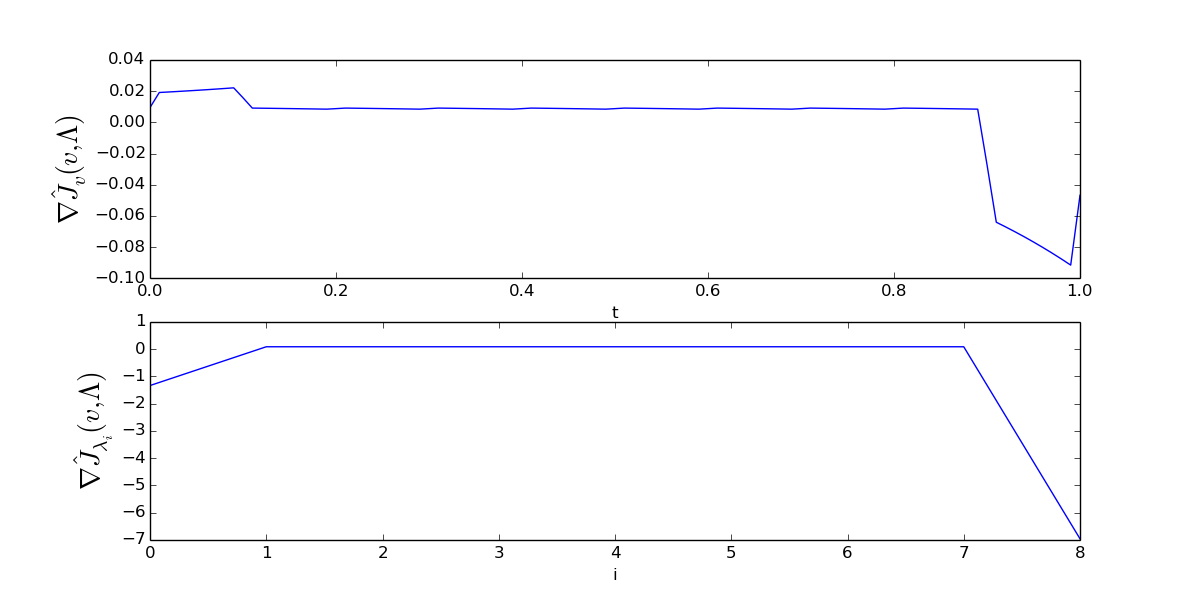
\includegraphics[scale=0.5]{pen_num_grad.png}
\caption{Plots showing the real and virtual part of the numerical gradient of the decomposed and penalized objective function of problem (\ref{test_J}-\ref{test_J}) found using formula (\ref{num_pen_grad_lam}-\ref{num_pen_grad_v}). Notice that the gradient has jumps between subintervals.}
\label{JGrad2}
\end{figure}
\section{Convergence Rate of Solver for the Non-Penalized Problem}
In section \ref{Taylor_sec} we demonstrated that our implementation of the gradients for different discretizations of the objective function introduced in theorem \ref{Theorem_num_grad} and \ref{Theorem_penalty_grad} satisfy the Taylor test. Since the discretized objective function $\hat J_{\Delta t}$ and its gradient pass the Taylor test, we expect that we can find the minimizer $\bar v$ of $\hat J_{\Delta t}$ by using an optimization algorithm. What we now want to find out, is if the minimizer of the discrete objective function converges towards the exact minimizer derived in section \ref{exact_sec}. We investigate this by solving optimal control problem (\ref{test_J}-\ref{test_E}) using both a Crank-Nicolson and an implicit Euler discretization. To measure the difference between exact optimal control $v_e$ and the numerical optimal control $v$ we look at the relative maximal difference between $v_e$ and $v$ for $t\in(0,T)$, meaning
\begin{align}
||v|| = \max_{k=1,...,n-1}|v_k| \label{inner_norm}
\end{align} 
We also look at the relative difference in objective function value between the controls. For both these measures, we calculate at what rate they converge to zero for decreasing $\Delta t$ values. The results for the implicit Euler discirization is found in table \ref{IE_convergence}, while Crank-Nicolson results are given in table \ref{CN_convergence}.
\begin{table}[!h]
\caption{Convergence of implicit Euler numerical sequential solver of optimal control problem. For each $\Delta t$ we find a numerical solution $v$ to problem (\ref{test_J}-\ref{test_E}) using an implicit Euler discretization and the L-BFGS optimization algorithm. We measre the difference between $v$ and the exact solution using the norm (\ref{inner_norm}), we also look at the fifference in objective function value between $v$ and $v_e$. In the columns (norm rate) and (functional rate), we report at which rate these error measures approch zero. We observe that the norm approches zero at a rate of one, while the difference in functional value converge towards zero at asecond order rate.} \label{IE_convergence}
\centering
\begin{tabular}{lrrll}
\toprule
{} $\Delta t$&    $\frac{||v_e-v||}{||v||}$ &  $\frac{\hat J(v_e)-\hat J(v)}{\hat J(v_e)}$ &   norm rate &    functional rate \\
\midrule
0.02000 &  0.2126 &  1.70e-02 &        -- &       -- \\
0.01000 &  0.1360 &  4.50e-03 & -0.64 & -1.92 \\
0.00100 &  0.0174 &  4.70e-05 & -0.89 & -1.98 \\
0.00010 &  0.0018 &  4.72e-07 &   -0.99 & -1.99 \\
0.00001 &  0.0002 &  4.72e-09 &  -1.00 & -1.99 \\
\bottomrule
\end{tabular}
\end{table}
Notice that the convergence rate of the norm difference in table \ref{IE_convergence} approaches one when $\Delta t$ tends to zero. This is consistent with what we would expect for a finite difference scheme of first order. We also notice that the difference in function value converges an order of one faster towards zero than the control difference.  
\begin{table}[!h]
\caption{Convergence of Crank-Nicolson numerical sequential solver of optimal control problem. The columns mean the same as in table \ref{IE_convergence}. For Crank-Nicolson we observe a second and a third order rate of convergence for the norm and functional difference when $\Delta t$ goes to zero.} \label{CN_convergence}
\centering
\begin{tabular}{lrrll}
\toprule
{} $\Delta t$&    $\frac{||v_e-v||}{||v||}$ &  $\frac{\hat J(v_e)-\hat J(v)}{\hat J(v_e)}$ &   norm rate &    functional rate \\
\midrule
0.02000 &  4.17e-02 &  2.30e-03 &       -- &       -- \\
0.01000 &  1.10e-02 &  3.38e-04 &  -1.91 & -2.77 \\
0.00100 &  1.18e-04 &  3.93e-07 & -1.96 & -2.93 \\
0.00010 &  1.42e-06 &  3.99e-10 & -1.92 & -2.99 \\
0.00001 &  1.48e-08 &  3.97e-13 & -1.98 &  -3.00 \\
\bottomrule
\end{tabular}
\end{table}
The results of table \ref{CN_convergence} show results similar to the ones in table \ref{IE_convergence}, however the convergence rates using a Crank-Nicolson scheme to discretize the ODEs are one order higher than the rates we got using implicit Euler. This is again expected since the Crank-Nicolson scheme is of order two. In both tables we observe that $\frac{\hat J(v_e)-\hat J(v)}{\hat J(v)}$ is always positive, which means that $\hat J(v_e)>\hat J(v)$. This makes sense, since $\hat J$ here means the discrete objective function, and $v$ is the minimum of this function, while $v_e$ is the minimum of the continuous objective function. One last remark concerns the choice of norm (\ref{inner_norm}). This norm excludes the values of $v$ and $v_e$ at $t=0$ and $t=T$. If these points are included, we do not see the convergence rates given in table \ref{IE_convergence} and \ref{CN_convergence}. 
\section{Verifying Function and Gradient Evaluation Speedups} \label{ver S sec}
In \ref{analysis sec} we derived the theoretical speedup for numerical gradient and objective function evaluation when decomposing the time-interval. It would now be interesting to check if the implementation achieves the theoretical speedup for our example problem (\ref{test_J}-\ref{test_E}). Now let us explain the experimental setting. A computer with 6 cores was used to verify the results of section \ref{analysis sec}. Having 6 cores means that we can do gradient and function evaluation for $N=1,2,...,6$ decompositions with different time step sizes $\Delta t$. For each combination of $N$ and $\Delta t$, we will run the function and gradient evaluations ten times, and then choose the the smallest execution time produced by the ten runs. The speedup is then calculated by dividing the sequential execution time by the parallel execution time. Tables \ref{Speed_table1}-\ref{speed_table_end} below shows runtime and speedup for both gradient and function evaluation for different $\Delta t$s and $N$s. All evaluations are done with control input $v=1$ and $\lambda_i=1$.  
\\
\begin{table}[!h]
\centering
\caption{$\Delta t=10^{-2}$}
\label{Speed_table1}
\begin{tabular}{lrrrr}
\toprule
{}$N$ &  functional time(s) &  gradient time(s) &  functional speedup &  gradient speedup \\
\midrule
1 &           0.00019 &          0.00021 &            1.000 &          1.000 \\
2 &           0.00020 &          0.00024 &            0.946 &          0.875 \\
3 &           0.00025 &          0.00028 &            0.780 &          0.753 \\
4 &           0.00030 &          0.00034 &            0.642 &          0.632 \\
5 &           0.00036 &          0.00039 &            0.544 &          0.547 \\
6 &           0.00045 &          0.00045 &            0.427 &          0.480 \\
\bottomrule
\end{tabular}
\end{table}
\begin{table}[!h]
\centering
\caption{$\Delta t=10^{-4}$}
\begin{tabular}{lrrrr}
\toprule
{} $N$&  functional time(s) &  gradient time(s) &  functional speedup &  gradient speedup \\
\midrule
1 &           0.0088 &          0.0150 &            1.000 &          1.000 \\
2 &           0.0044 &          0.0077 &            1.983 &          1.946 \\
3 &           0.0031 &          0.0053 &            2.838 &          2.816 \\
4 &           0.0024 &          0.0040 &            3.582 &          3.677 \\
5 &           0.0020 &          0.0033 &            4.267 &          4.457 \\
6 &           0.0019 &          0.0030 &            4.519 &          4.978 \\
\bottomrule
\end{tabular}
\end{table}
\begin{table}[!h]
\centering
\caption{$\Delta t=10^{-5}$}
\begin{tabular}{lrrrr}
\toprule
{} $N$&  functional time(s) &  gradient time(s) &  functional speedup &  gradient speedup \\
\midrule
1 &           0.0874 &          0.1548 &            1.000 &          1.000 \\
2 &           0.0435 &          0.0756 &            2.006 &          2.046 \\
3 &           0.0302 &          0.0521 &            2.888 &          2.971 \\
4 &           0.0223 &          0.0386 &            3.913 &          4.003 \\
5 &           0.0180 &          0.0314 &            4.848 &          4.921 \\
6 &           0.0161 &          0.0269 &            5.425 &          5.755 \\
\bottomrule
\end{tabular}
\end{table}
\begin{table}[!h]
\centering
\caption{$\Delta t=10^{-7}$}
\label{speed_table_end}
\begin{tabular}{lrrrr}
\toprule
{}$N$ &  functinal time(s) &  gradient time(s) &  functional speedup &  gradient speedup \\
\midrule
1 &           8.350 &         14.930 &            1.000 &          1.000 \\
2 &           4.200 &          7.233 &            1.987 &          2.064 \\
3 &           2.932 &          5.033 &            2.847 &          2.966 \\
4 &           2.190 &          3.861 &            3.812 &          3.866 \\
5 &           1.796 &          3.089 &            4.647 &          4.833 \\
6 &           1.524 &          2.599 &            5.479 &          5.744 \\
\bottomrule
\end{tabular}
\end{table}
\\
\\
Since the parallel algorithm has some overhead, we do not expect any improvements for small problems. This is reflected in the above results, where we for $\Delta t = 10^{-2}$ see an increased execution time when running function and gradient evaluation in parallel. For $\Delta t = 10^{-4}$ we see only a modest speedup, that is significantly lower than the expected speedup from section \ref{analysis sec}. For $\Delta t \leq 10^{-5}$, however we see speedup results in line with what we expect from the theory.  
\section{Consistency of the Penalty Method} \label{consistency_sec}
When we introduced the penalty method in section \ref{penalty_sec}, we also presented a result showing that the iterates $\{v^k\}$ stemming from the penalty algorithmic framework converged towards the solution of the non-penalized problem $v$ if for all $k$ $(v^k,\Lambda^k)$ is the exact global minimizer of $\hat J_{\mu_k}$. We can write this up as:
\begin{align*}
\lim_{k\rightarrow\infty} v^k = v 
\end{align*}  
An alternative way of looking at this, is to let $v^{\mu}$ be the minimizer of $\hat J_{\mu}$, and instead write the above limit as:
\begin{align}
\lim_{\mu\rightarrow\infty} v^{\mu} = v \label{mu con}
\end{align}
The interpretation of the above limit, is that solving the penalized problem with an ever increasing penalty parameter $\mu$ should result in a solution that is getting closer and closer to the solution of the non-penalized problem. This means that the penalty algorithm is consistent, since it produces the same solution as the ordinary non-decomposed problem. It is therefore worth checking if the implementation of the penalized problem actually has the property (\ref{mu con}). We investigate this by comparing the solution we get by decomposing and then applying the penalty method on problem (\ref{test_J}-\ref{test_E}) with the solution we get by solving the undecomposed problem. 
\\
\\
We discretize (\ref{test_J}-\ref{test_E}) using Crank-Nicolson and the trapezoid rule for two different time steps. First we let $\Delta t = 10^{-2}$ and apply the penalty method for $N=2$ and $N=10$ decompositions, we then let $\Delta t = 10^{-3}$ and test the penalty method on $N=2$ and $N=7$ decompositions. We use different metrics to compare the non-penalized and penalized solutions, so that we better see how the solution of the penalized problem behaves when we solve it for an increasing sequence of $\mu$ values. We define the metrics as follows:
\begin{align}
\textrm{Realtive objective function difference:}\quad \Delta \hat J &= \frac{\hat{J}(v_{\mu})-\hat{J}(v)}{\hat{J}(v)}.\label{mes1}\\
\textrm{Realtive penalized objective function difference:}\quad \Delta \hat J_{\mu} &= \frac{\hat{J}_{\mu}(v)-\hat{J}_{\mu}(v_{\mu})}{\hat{J}_{\mu}(v)}.\\
\textrm{Relative control $L^2$-norm difference:}\quad \Delta v&=\frac{||v_{\mu}-v||_ {L^2}}{||v||_{L^2}}. \\
\textrm{Maximal jump in decomposed state equation:}\quad \Delta y&= \sup_i\{y_{k_i}^i-y_{k_i}^{i+1}\}.\label{mes4}
\end{align}
Notice that both $\Delta\hat J$ and $\Delta \hat J_{\mu}$ should be grater than $0$, since $v$ and $v_{\mu}$ are the minimizers of $\hat J$ and $\hat J_ {\mu}$. The measure of jumps in the state equation $\Delta y$ is added to check that the penalty solution approaches a feasible solution in context of the continuity constraints (\ref{Extra constraints}). The results of the above detailed experiment are presented through logarithmic plots in figure \ref{Cons1_fig} and \ref{Cons2_fig}. In addition to the already mentioned measures, these plots include the error between the exact solution $v_e$ and the sequential error $v$ as a reference.
\\
\begin{figure}[!h]
\centering
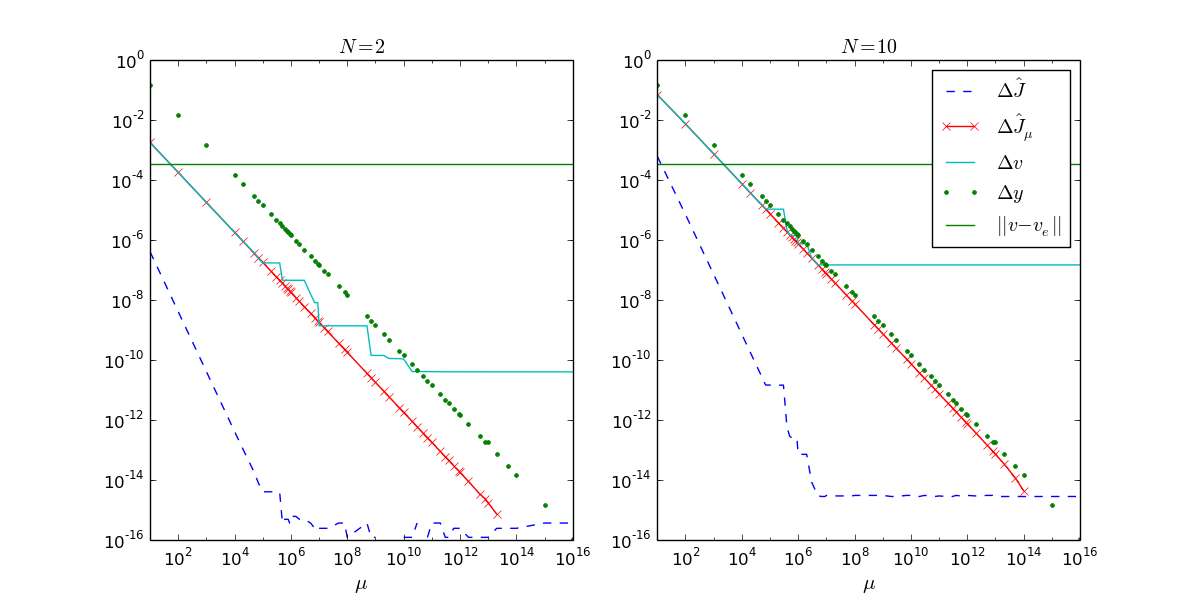
\includegraphics[scale=0.5]{consistency1.png}
\caption{Logarithmic plot showing how the minimizer of $\hat J_{\mu}$ develops in comparison to the minimizer of $\hat J$ for increasing penalty parameter $\mu$, when solving problem (\ref{test_J}-\ref{test_E}) with $\Delta t = 10^{-2}$. The measures plotted are defined in (\ref{mes1}-\ref{mes4}). The horizontal line $||v-v_e||$ is the accuracy of the unpenalized sequential solution. The left plot shows results of using $N=2$ decompositions of the time interval, while on the right we have used $N=10$ decompositions.}
\label{Cons1_fig}
\end{figure}
\noindent
\begin{figure}[!h]
\centering
\includegraphics[scale=0.5]{consistency2.png}
\caption{Same as figure \ref{Cons1_fig}, only now $\Delta t = 10^{-3}$.}
\label{Cons2_fig}
\end{figure}
\noindent
\\
The plots in figure \ref{Cons1_fig} and \ref{Cons2_fig} all show a similar picture, and we observe that all measures decrease when the penalty parameter is increased. Still there are several parts of the plots worthy of note. The measure $\Delta\hat J$ related to the unpenalised objective function is the value that converges to zero the fastest. If we look at the values of $\Delta\hat J$ before the machine precision is reached we see that $\Delta \hat J$ is proportional to $\frac{1}{\mu^2}$. The convergence rate of $\Delta\hat J$ for $\Delta t=10^{-2}$ and $N=2$ is shown in table \ref{Cosn_rate_table} together with the convergence rate of $\Delta v$. $\Delta v$ and the other measures converge to zero at a rate of one, however we see that the relative error $\Delta v$ between the controls $v$ and $v_{\mu}$ stops to decrease long before the machine precision is reached. It seems that this barrier is hit around the same time as $\Delta\hat J$ approaches machine precision. The reason for this probably is that small changes in the control $v_{\mu}$ no longer registers in $\hat J_{\mu}$. It is therefore difficult to find an appropriate step length in the line search method, and this again means that we no longer are capable of finding the exact global minimizer of $\hat J_{\mu}$. If we remember theorem \ref{consistency theorem} from section \ref{penalty_sec} the sequence $\{v^{k}\}$ only converge toward $v$ if for all $k$ $(v^{k},\Lambda^k)$ is the global minimizer of $\hat J_{\mu}$. The results of figure \ref{Cons1_fig} and \ref{Cons2_fig} is therefore in line with the claim of theorem \ref{consistency theorem}.
\\
\\
Unlike $\Delta v$, $\Delta\hat J_{\mu}$ and $\Delta y$ continue to decrease steadily towards zero, even after $\Delta \hat J$ has hit machine precision. The $\Delta\hat J_{\mu}$ and $\Delta y$ metrics are both related to the $\frac{\mu }{2}\sum_{i=1}^{N-1}(y^i(T_{i})-\lambda_i)^2$ term, which is the part that enforces the continuity constraints (\ref{Extra constraints}). This is again in line with the theory presented in section \ref{penalty_sec}. There we stated theorem \ref{feasible theorem}, which guaranteed that the iterates $\{(v^{k},\Lambda^k)\}$ of the penalty method would converge to a feasible point when $\mu_k$ tended to infinity. 
\begin{table}[!h]
\centering
\caption{Convergence rates for $\Delta t=10^{-2}$ and $N=2$. The second and third column show how difference in objective function value and norm between the numerical solution of the penalized problem $v^{\mu}$ and the solution of the unpenalized problem $v$ develop for increasing $\mu$ values. The two last columns show at what rate these differences approach zero. We see that $\Delta \hat J$ is proportional to $\mu^{-2}$, while $\Delta v$ is proportional to $\mu^{-1}$. Notice how the $\Delta v$ stops to decrease at around the same time as $\Delta \hat J$ hits machine precision.}
\label{Cosn_rate_table}
\begin{tabular}{lrrll}
\toprule
{} $\mu$&  $\Delta \hat J$ &   $\Delta v$ &        $\Delta \hat J$ rate &        $\Delta v$ rate \\
\midrule
1e+01 &      4.10e-07 & 1.79e-03 &            -- &            -- \\
1e+02 &      4.11e-09 & 1.79e-04 & -1.99 & -0.999 \\
1e+03 &      4.12e-11 & 1.79e-05 & -1.99 & -1.000 \\
1e+04 &      4.13e-13 & 1.79e-06 & -1.99 & -0.999 \\
1e+05 &      4.04e-15 & 1.73e-07 & -1.99 & -0.985 \\
4e+05 &      3.80e-15 & 1.71e-07 & -0.11 & -0.008 \\
5e+05 &      3.67e-16 & 4.54e-08 & -10.4 & -5.96 \\
\bottomrule
\end{tabular}
\end{table}
